\documentclass[a4j,10pt,twocolumn]{abstract}
%\documentclass[a4j,9pt,twocolumn]{abstract}
\usepackage{graphicx}
\usepackage[varg]{txfonts}
%%% \begin{document}の前に,各エントリーを記述する

\setlength\textfloatsep{10pt}     %図と本文の間
\setlength\abovecaptionskip{0pt} %図とキャプションの間
\setlength\floatsep{0pt} %図同士の間

\title{Scalable Parallel Computing \\ on NoC-based Embedded Many-Core Platform}	% 論文のタイトル

\author{丸山雄也} 		% 著者
\studentid{29C16090} 	% 学籍番号
\lab{潮}		% 研究室名

% 英語なら以下2行を定義
\englishtitle
\jptitle{NoCベース組込み向けメニーコアにおけるスケーラブルな並列計算}  % 日本語のタイトル

\begin{document}
\absttitle 		% 表題の出力

\section{緒論}
% 近年,組込みシステムの要求する高い計算性能や電力効率を背景に,次世代計算機としてメニーコア・プロセッサが注目を集めている.
近年,自動運転を始めとする様々な組込みシステムにおいて,低消費電力での高い計算性能が求められている.
メニーコア・プロセッサはそれらの要件を満たすことから,実用化に向けた様々な研究 \cite{BURGIO20172992}, \cite{de2013clustered2} の対象となっているが,基礎評価や実用性の評価は不十分である.
さらに,大規模・複雑化する組込みシステムに対応するため,メニーコア向けソフトウェア開発の生産性向上が要求されている.

本研究では,Network-on-Chip (NoC) をベースとしたメニーコア・プロセッサを用いた基礎評価や自動運転アプリケーションの並列化を行い,構造化されたメッセージ通信を提供するミドルウェア及びそのソフトウェア開発フレームワークを提案する.
基礎評価や実アプリケーションの並列化により並列計算のスケーラビリティやメニーコア・プロセッサの実用性を示し,提案フレームワークでは,メニーコア・プロセッサ向けソフトウェア開発の効率化を図る.

\section{組込み向けメニーコア・プロセッサ}
本研究では,組込み向けメニーコア・プロセッサとしてKalray社のMPPA-256 \cite{de2013clustered2} を対象とする.
MPPA-256 は,256個のコアを持つメニーコア・プロセッサであり,多数のコアでの計算を実現する為にNoCによるクラスタ構成を採用する.
メモリを共有した16個のコアを1つのクラスタとし,16個のクラスタ同士がチップ上でネットワークを構成し,相互に通信を行う.
NoCを用いたクラスタ構成により,コア数増加に伴い頻繁するメモリへのアクセス競合を解消し,コア数の増加を実現する.

\section{提案フレームワーク}
提案フレームワークでは,組込みシステムのメモリ制約下でも動作可能なメニーコア向けメッセージ通信ミドルウェア(ROS-lite)を提供し,図\ref{fig:model}に示す開発手法により開発効率の向上を図る.
ROS-liteでは,構造化されたメッセージをメニーコア・プロセッサ内で動作するプログラム同士でPublish/Subscribeモデルによって通信する機能を提供する.
メッセージ通信APIは,ミドルウェア内部でNoCを介した通信APIに置き換えられ,ハードウェアに依存するソースコード記述をユーザから抽象化する.
フレームワーク全体としては,プログラムをコアへ割り当てるソースコード等の自動生成機能によって開発効率の向上を行う.

そして,多くのロボットソフトウェア開発で用いられているRobot Operating System (ROS)のソースコードをそのままメニーコア・プロセッサ上で動作させることを可能としており,プログラムの再利用性を高める.

\section{評価}
本研究では,NoCベース組込み向けメニーコア・プロセッサによるNoC通信の遅延評価やマイクロベンチマークによるスケーラビリティの評価,実アプリケーションの並列化による実行時間の評価を行った.
図\ref{fig:eval}は,自動運転アプリケーションにおける高精度3次元地図内での自己位置推定処理の実行時間を示したものである.
並列化により実行時間が短縮され,多くの自動運転システムでデッドラインとされる100msを下回る結果となった.

\section{結論}
本研究では,MPPA-256を用いたNoCベース組込み向けのメニーコア・プロセッサによる基礎評価および実アプリケーションの並列化により,NoCの通信特性や並列計算のスケーラビリティ,並列化の実用性を明らかにした.
さらに,NoC上でのメッセージ通信APIの提供により,ROSのソースコードをメニーコア・プロセッサ上で容易に開発・実行するソフトウェア開発フレームワークを提案した.
今後は,自動運転アプリケーションのさらなる移植や並列化,ROS-liteのリアルタイム性向上や対応機能の拡張が課題として挙げられる.

\begin{figure}[t]
    \centering
    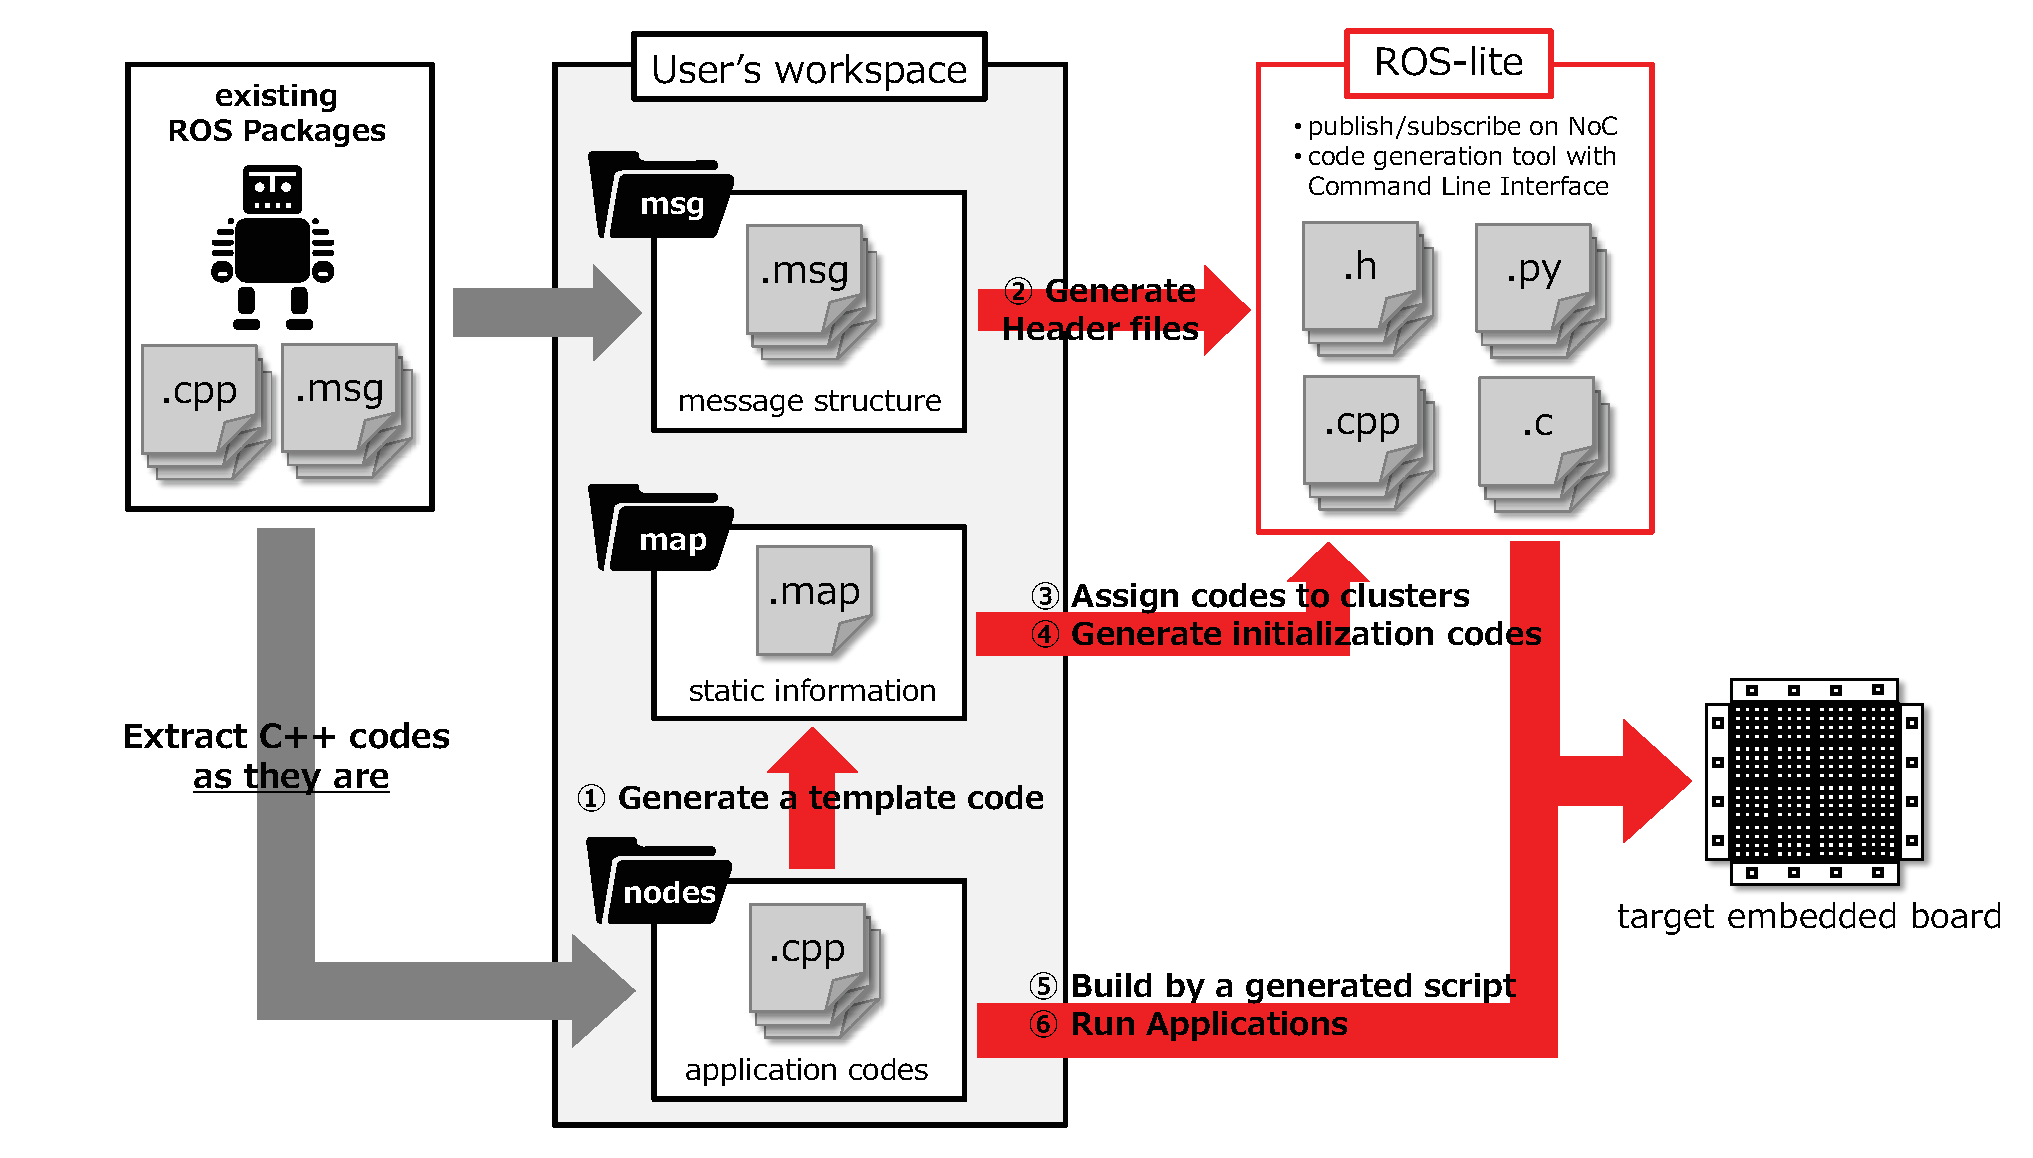
\includegraphics[width=0.9\linewidth]{../../figure/roslite/system_model.eps}
    \caption{\label{fig:model}
        ROS-liteによるメニーコア向けソフトウェア開発の流れ}
\end{figure}

\begin{figure}[t]
    \centering
    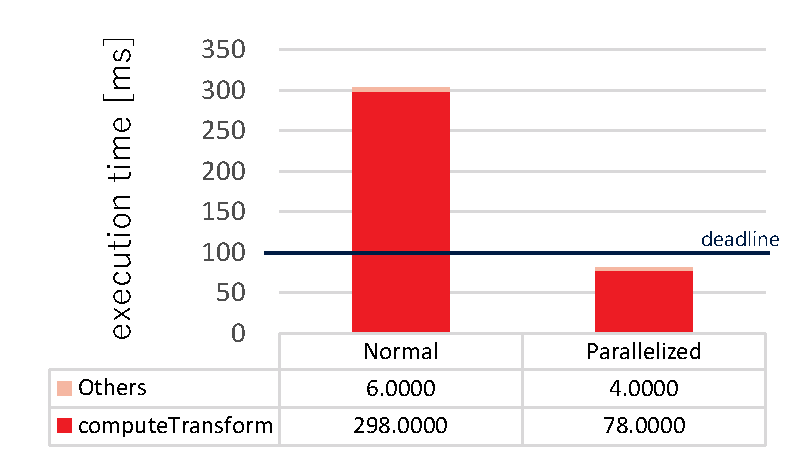
\includegraphics[width=0.9\linewidth]{../../figure/BarGraph_ndt_matching.eps}
    \caption{\label{fig:eval}
    自動運転における車両の自己位置推定処理の並列化}
\end{figure}

\bibliographystyle{junsrt}
\bibliography{../reference}
  
% \begin{thebibliography}{1}
% \bibitem{} 
% \end{thebibliography}

\newpage
\pagebreak
\end{document}
